\begin{frame}
  \frametitle{Experiment result}
  \begin{itemize}
  \item{Environment
  \begin{itemize}
  \setlength\itemsep{0.5em}
  \item{Platform:Arch Linux 64 bit, GCC 6.1.1 compiler}
  \item{Skylake i7-6600U CPU @ 3GHz}
  \item{64 bit multiplication (mul, mulx): 1 op/cycle}
  \item{64 bit addition/subtraction (add, sub): 4 op/cycle}
  \item{64 bit addition with carry (adc, adcx, adox): 1 op/cycle}
  \item{Carry addition only: peak performance of 2 ops/cycle
  {\raise.17ex\hbox{$\scriptstyle\sim$}} 6 Gops/s on 1 core}
  \item{Compilation flags: -fomit-frame-pointer -O3 -mavx2 -mbmi2 -madx}
  \end{itemize}
}
  \setlength\itemsep{1.5em}
  \end{itemize}
\end{frame}
\begin{frame}
\begin{figure}\flushleft		
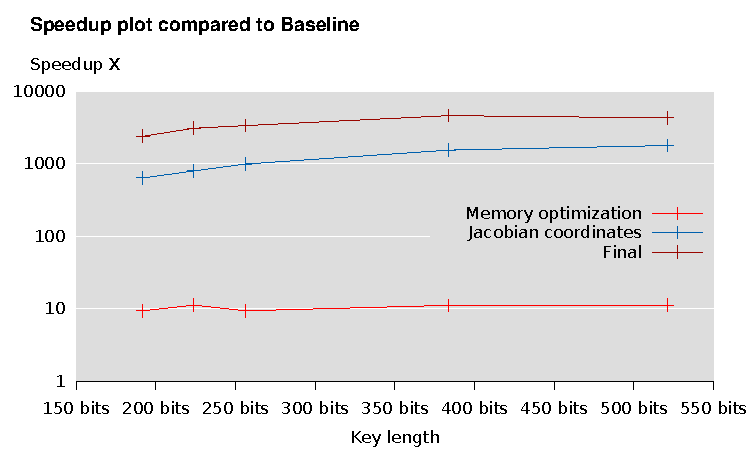
\includegraphics[scale=0.9, trim={0 0 0 0}]{speedup}		
\end{figure}
\end{frame}
\begin{frame}
\begin{figure}\flushleft		
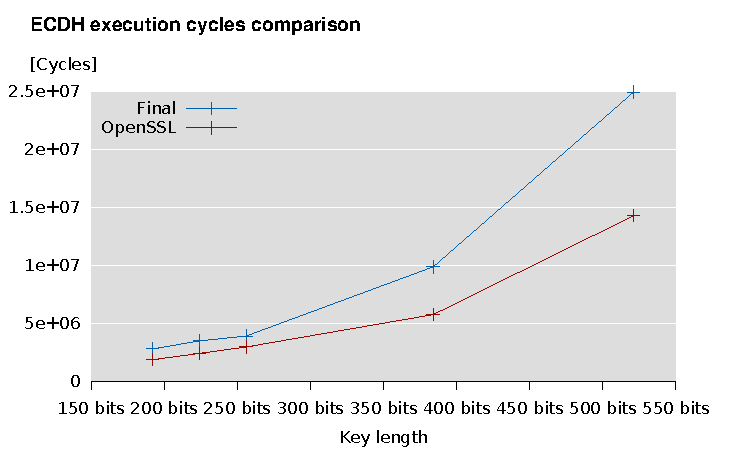
\includegraphics[scale=0.9, trim={0 0 0 0}]{ecdh}		
\end{figure}
\end{frame}
\begin{frame}
\begin{figure}\flushleft		
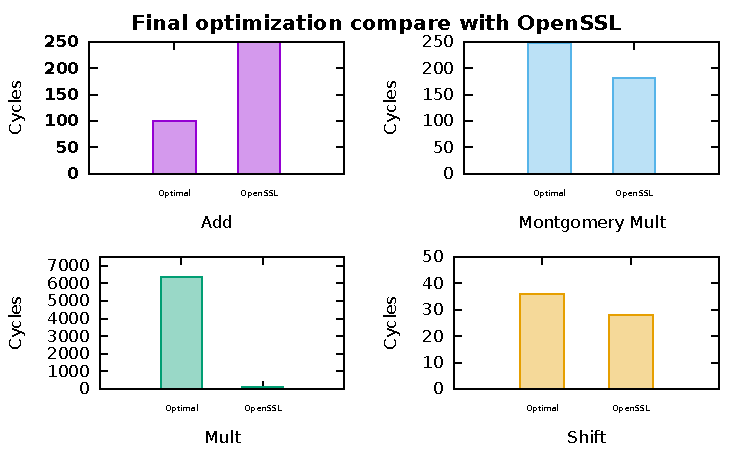
\includegraphics[scale=0.9, trim={0 0 0 0}]{openssl}		
\end{figure}
\end{frame}
\begin{frame}
\begin{figure}\flushleft		
\includegraphics[scale=0.9, trim={0 0 0 0}]{perfplot1}		
\end{figure}
\end{frame}
\begin{frame}
\begin{figure}\flushleft		
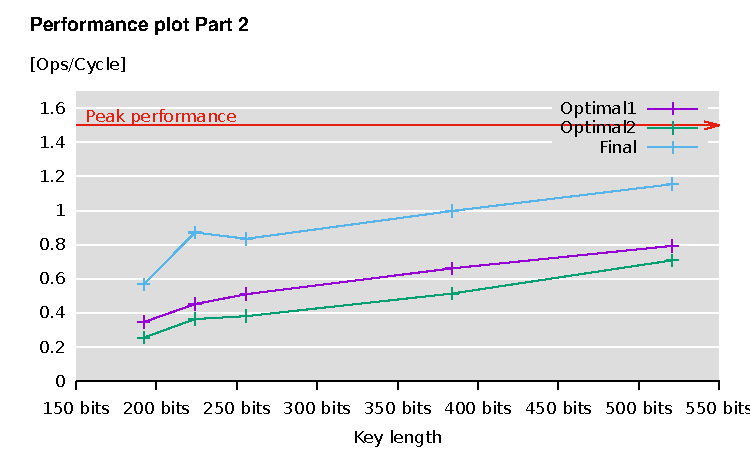
\includegraphics[scale=0.9, trim={0 0 0 0}]{perfplot2}		
\end{figure}
\end{frame}
\begin{frame}
\begin{figure}\flushleft		
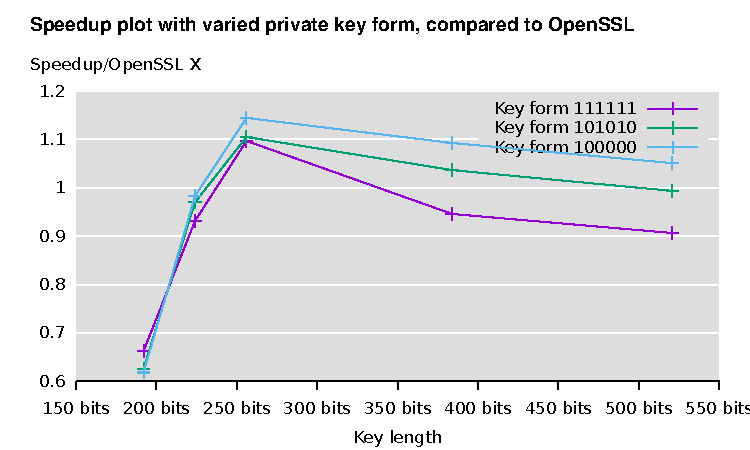
\includegraphics[scale=0.9, trim={0 0 0 0}]{keysize}		
\end{figure}
\end{frame}